\documentclass[a4paper,12pt]{article}
\usepackage[utf8]{inputenc}
\usepackage[T1]{fontenc}
\usepackage[french]{babel}
\usepackage[right=2.5cm, left=2.5cm]{geometry}
\usepackage[ddmmyyyy]{datetime}
\usepackage[table]{xcolor}
\usepackage{lmodern,mathptmx,changepage,titlesec,hyperref,listings,lstautogobble,graphicx,array,longtable,multirow,lipsum,tikz,shorttoc,enumitem}
\usetikzlibrary{arrows,automata}
\usetikzlibrary{positioning}

\renewcommand{\rmdefault}{\sfdefault} %Utilisation de la police sans-serif ("Computer Modern Sans") pour la police roman
\renewcommand{\ttdefault}{pcr} 	%Utilisation d'une police "CourrierNew" pour la police monospaced (pour faire un listing manuel)
\linespread{1.15}				%Interligne

%Utilisation de liens colorés en bleu et soulignés
\hypersetup{colorlinks=true, urlcolor=blue, urlbordercolor=blue, linkcolor=black, linkbordercolor=white}
\makeatletter \Hy@AtBeginDocument{\def\@pdfborder{0 0 1} \def\@pdfborderstyle{/S/U/W 1}}\makeatother

\titlespacing*{\section} {0cm}{7ex plus 1ex minus .2ex}{1.5ex plus .2ex}
\titlespacing*{\subsection} {0cm}{4.5ex plus 1ex minus .2ex}{1.5ex plus .2ex}
\titleformat*{\section}{\huge\bfseries}
\titleformat*{\subsection}{\Large\bfseries}
\titleformat*{\subsubsection}{\normalsize\bfseries}

\definecolor{darkgreen}{rgb}{0,0.8,0}
\definecolor{mygray}{rgb}{0.93,0.93,0.93}
\definecolor{mymauve}{rgb}{0.58,0,0.82}
\lstset{	
	basicstyle=\small\ttfamily,
	backgroundcolor=\color{mygray},
	breaklines=true,
	breakatwhitespace=true,
	postbreak=\raisebox{0ex}[0ex][0ex]{\ensuremath{\color{red}\hookrightarrow\space}},
	tabsize=3,
	frame=none,
	rulecolor=\color{black},
	keywordstyle=\color{blue}\bfseries,
	stringstyle=\color{orange},
	showstringspaces=false,
	commentstyle=\footnotesize\color{darkgreen},
	keepspaces=true,
	extendedchars=true,
	numbers=left,
	numberstyle=\tiny\color{lightgray},
	stepnumber=1,
	escapeinside={(@}{@)},
	autogobble=true,
	literate=
		{á}{{\'a}}1 {é}{{\'e}}1 {í}{{}}1 {ó}{{\'o}}1 {ú}{{\'u}}1
		{Á}{{\'A}}1 {É}{{\'E}}1 {Í}{{\'I}}1 {Ó}{{\'O}}1 {Ú}{{\'U}}1
		{à}{{\`a}}1 {è}{{\`e}}1 {ì}{{\`i}}1 {ò}{{\`o}}1 {ù}{{\`u}}1
		{À}{{\`A}}1 {È}{{\'E}}1 {Ì}{{\`I}}1 {Ò}{{\`O}}1 {Ù}{{\`U}}1
		{ä}{{\"a}}1 {ë}{{\"e}}1 {ï}{{\"i}}1 {ö}{{\"o}}1 {ü}{{\"u}}1
		{Ä}{{\"A}}1 {Ë}{{\"E}}1 {Ï}{{\"I}}1 {Ö}{{\"O}}1 {Ü}{{\"U}}1
		{â}{{\^a}}1 {ê}{{\^e}}1 {î}{{\^i}}1 {ô}{{\^o}}1 {û}{{\^u}}1
		{Â}{{\^A}}1 {Ê}{{\^E}}1 {Î}{{\^I}}1 {Ô}{{\^O}}1 {Û}{{\^U}}1
		{œ}{{\oe}}1 {Œ}{{\OE}}1 {æ}{{\ae}}1 {Æ}{{\AE}}1 {ß}{{\ss}}1
		{ç}{{\c c}}1 {Ç}{{\c C}}1 {ø}{{\o}}1 {å}{{\r a}}1 {Å}{{\r A}}1
		{€}{{e}}1 {£}{{\pounds}}1 {«}{{\guillemotleft}}1
		{»}{{\guillemotright}}1 {ñ}{{\~n}}1 {Ñ}{{\~N}}1 {¿}{{?`}}1
}

%Redéfinition de la taille de \Huge pour le titre du document
\makeatletter\renewcommand\Huge{\@setfontsize\Huge{37pt}{40}}\makeatother
\date{\today}

\title{\vspace{\fill}\textbf{\Huge Cahier des Charges}}
\author{
	Sonny Klotz - Jean-Didier Pailleux - Malek Zemni
	\vspace{2em}\\
	\textit{Interface de chargement, de contrôle}\\\textit{et d’analyse statistique des données}\\\textit{pour la constitution d’un graphe de flux}
	\vspace{2em}
}


\begin{document}
\pagenumbering{gobble}\clearpage
\maketitle\vspace{13em}
\begin{center}
\includegraphics[scale=0.7]{logo.png}\end{center}
\begin{flushright}Module \textit{Projet}\end{flushright}
\newpage
\tableofcontents
\newpage\clearpage\pagenumbering{arabic}

	\section*{Introduction}
		Ce projet s'inscrit dans le cadre du module \textit{Projet} de la licence informatique de l'UVSQ. Le sujet qu'on nous a remis a été proposé par l'entreprise DCbrain. Notre travail va être décrit au préalable dans ce cahier des charges en plusieurs points.\\
		Dans les deux premières parties, on va décrire le contexte et l'environnement dans lequel va s'inscrire notre système. Ensuite, les exigences vont permettre de détailler les fonctionnalités l'application. Finalement, la dernière partie s'intéressera à notre démarche de travail.
	
	\section{Motivations du projet}
		\subsection{But du projet}
			\subsubsection{Contexte du projet}
			De nos jours, les masses de données collectées sont de plus en plus importantes. L'objectif principal de cette collecte de données est d'en extraire une valeur ajoutée. Or, ces données à l'état brut sont difficilement exploitables dû à leur volume et à leur complexité.\\
			Notre produit correspond au travail indispensable d'analyse de ces données, afin de faciliter leur exploitation.
			\subsubsection{Objectif du projet}
			Ce projet a pour but de fournir aux utilisateurs une application web qui se chargera d'une part de structurer les données, les analyser et les visualiser, et d'autre part de préparer ces données pour un chargement via des API. Ces données supplémentaires permettront d'alimenter leur base de données dans le but de mieux prévenir la présence d'anomalie sur les réseaux physique.
		
		\subsection{Parties prenantes}
			\subsubsection{Maître d'ouvrage}
			Notre interface de contrôle, de chargement, et d'analyse de données est développée pour l'entreprise \textbf{DCbrain}.\\
			Le projet a été lancé en collaboration avec l'\textbf{UVSQ}.\\
			Ils suivent ce projet et sont amenés à décider des grandes orientations prisent pour son élaboration.
			
			\subsubsection{Client}
			DCbrain est l'entreprise qui va bénéficier des paquets finaux après leur développement. Le projet étant un produit qui va leur permettre de mieux comprendre ce qui se passe sur leurs réseaux.\\
			Cette entreprise spécialisée dans l'analyse de données collectées à partir de réseaux physiques, cherche à développer un outil de visualisation préliminaire de données.\\
			Notre travail doit donc pouvoir être utilisé par DCbrain pour renforcer leur application.
			
			\subsubsection{Autre partie prenante}
			Les industriels clients de DCbrain sont des parties prenantes indirectes. Leur rôle consistant à fournir les données à la startup pour l'analyse de données. Le projet est motivé par le besoin de gérer leurss réseaux physiques plus efficacement.
			
			\subsubsection{Synthèse}
			\begin{center}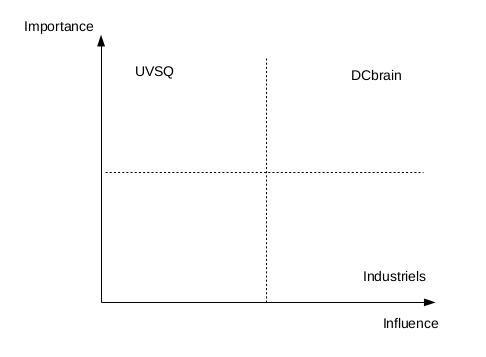
\includegraphics[scale=0.8]{diagPP.png}\end{center}
			\textbf{Remarque :} les différents acteurs seront décrits plus précisément dans la partie \textit{Périmètre de l'ouvrage}.
			
		\subsection{Utilisateurs du produit}
		En premier lieu, l’application va servir aux membres de DCbrain étant donné que leurs clients industriels (Total, ERDF,…) leur fournissent les fichiers CSV, afin qu’ils puissent appliquer des analyses descriptives sur les données dans le but de repérer des anomalies sur les réseaux de ces derniers. Puis en second lieu, DCbrain va déployer l'application pour ses clients, dans ce cas les membres de ces organismes deviendront des utilisateurs.\\


	\section{Contraintes sur le Projet}
		\subsection{Contraintes imposées}
			\subsubsection{Contraintes sur la conception :}
				\begin{center}\begin{longtable}{|>{\centering}m{3cm}|>{\raggedright\arraybackslash}m{10cm}|}			
				\hline \multicolumn{1}{|c}{\textbf{Contrainte}} & \multicolumn{1}{|c|}{\textbf{Fiche}} \\
				\hline 	1. Le produit doit fournir une application web &
						\begin{description}[style=unboxed,leftmargin=0.2cm]
						\item{\textbf{Description :}} notre produit sera une application fonctionnant sur un navigateur web, appelée \textbf{\textit{applet}}.
						\item{\textbf{Justification :}} assure une très grande portabilité et fournit à l'utilisateur une interface interactive.
						\item{\textbf{Critère de satisfaction :}} on peut lancer l'application sur un navigateur web.
						\end{description}\\
				\hline 2. Le produit doit être développé avec un langage de programmation compatible avec l'analyse de données &
						\begin{description}[style=unboxed,leftmargin=0.2cm]
						\item{\textbf{Description :}} le langage de programmation choisi doit inclure des bibliothèques qui permettent d'analyser les données (taches de data mining et de machine Learning).
						\item{\textbf{Justification :}} permettre une analyse de données efficace.
						\item{\textbf{Critère de satisfaction :}} on peut effectuer une analyse descriptive de données.
						\end{description}\\
				\hline 3. Le produit doit fournir une API d'analyse de données en sortie &
						\begin{description}[style=unboxed,leftmargin=0.2cm]
						\item{\textbf{Description :}} l'application doit intégrer des API d'analyse descriptive de données qui pourront être livrées en sortie au client.
						\item{\textbf{Justification :}} permettre une réutilisabilité des fonctionnalités majeures du produit.
						\item{\textbf{Critère de satisfaction :}} on peut exporter une API d'analyse de données en sortie.
						\end{description}\\
				\hline
				\end{longtable}\vspace{1em}\end{center}
				
			\subsubsection{Environnement de fonctionnement :}
				Le produit va fournir une application web ou \textbf{\textit{applet}}. L'environnement technologique de ce genre d'application
				sont les navigateurs web. Ces navigateurs web jouent le rôle d'interface entre l'utilisateur et l'application.
				
				\begin{center}\begin{tikzpicture}\begin{scope}[xscale=2,yscale=1.5]	
					\node (USR) at (-3,0) [rectangle,draw] {\begin{tabular}{c}Utilisateur\end{tabular}};
					\node (NAV) at (0,0) [rectangle,draw,fill=blue!25] {\begin{tabular}{c}Navigateur web\end{tabular}};
					\node (APP) at (3,0) [rectangle,draw] {\begin{tabular}{c}Application\end{tabular}};
					\path[->,>=stealth'] (USR) edge[bend left=0] node[anchor=south,above]{Accès à l'hôte} (NAV);
					\path[->,>=stealth'] (NAV) edge[bend left=13] node[anchor=south,above]{Intégration de l'application} (APP);
				\end{scope}\end{tikzpicture}\end{center}
					
				Le produit doit donc être compatible avec tous les navigateurs web bureau (pas de version mobile exigée) prenant en charge les fonctionnalités des dernières versions \textbf{\textit{HTML5}} et \textbf{\textit{CSS3}}, par exemple \textbf{\textit{Google Chrome}} et \textbf{\textit{Mozilla Firefox}}.
				
			\subsubsection{Applications partenaires :}
				Le produit va fournir une API en sortie. Il doit donc prendre en compte de l'environnement d'intégration de cette API, c'est à dire que cette API doit être compatible avec les outils du client, l'entreprise DCbrain.
				
			\subsubsection{Temps dont disposent les développeurs du projet :}
				Le produit doit être rendu avant le 26/05/2017.
				
			\subsubsection{Budget du projet :}
				La réalisation du produit n'exige pas de ressources financières. Aucun budget n'est donc nécessaire.
		
		\subsection{Glossaire et conventions de dénomination}
			\begin{description}[style=unboxed,leftmargin=0.2cm]
				\item\textbf{Maître d'ouvrage :} entité porteuse du besoin, définissant l'objectif et les exigences du projet, attendant la réalisation d'un produit, appelé ouvrage.
				\item\textbf{Maître d'œuvre :} entité retenue par le maître d'ouvrage pour réaliser l'ouvrage.
				\item\textbf{Big data :} ensembles de très gros volumes de données traitées et exploitées pour en tirer des informations.
				\item\textbf{Machine Learning :} méthodes automatisables offrant la possibilité à une machine d'évoluer grâce à un processus d'apprentissage à partir des données.
				\item\textbf{Réseaux physiques :} réseaux industriels, de fluide, de distribution (par exemple réseau électrique).
				\item\textbf{Capteurs IOT :} capteurs \textit{Internet of Things} (internet des objets) déployés sur des réseaux physiques afin d'y collecter des données.
				\item\textbf{Graphe de flux :} graphes représentant les données liées au flux du réseau.
				\item\textbf{CSV :} \textit{Comma-separated values}, format de fichier ouvert représentant des données tabulaires sous forme de valeurs séparées par des virgules.
				\item\textbf{ADD :} \textit{Analyse Descriptive de Données}, ensemble de techniques de statistique descriptive. Elle consiste à regrouper les données de manière homogène et fournir des descriptions synthétiques de comportements globaux.
				\item\textbf{ADD unidimensionnelle :} appelée aussi ADD univariée, elle correspond aux techniques manipulant un seul critère du système étudié.
				\item\textbf{ADD multidimensionnelle :} ADD où les intéractions entre différents critères d'études sont pris en compte pour décrire le jeu de données dans son ensemble.
				\item\textbf{Applet :} application qui s'exécute dans la fenêtre d'un navigateur web.
				\item\textbf{API :} \textit{Application Programming Interface}, constituent les paquets utilisables par les développeurs (intégrés), qu'on va livrer au client en plus de l'application elle-même.
				\item\textbf{Drag\&Drop :} glisser et déposer un fichier dans une fenêtre.
				\item\textbf{Structure 1 :} structure contenant les données du fichier, le nombre de lignes et le nombre de colonnes.
				\item\textbf{Structure 2 :} structure contenant 3 informations sur chaque colonne : le type, le rôle et les positions des données erronées.
			\end{description}
			
	\section{Exigences fonctionnelles}
	
		\subsection{Périmètre de l'ouvrage}
			Deux parties prenantes vont interagir avec notre système :
			\begin{itemize}
			\item Les industriels : ce sont les détenteurs des réseaux physiques et des données mesurées grâce aux capteurs IoT, clients de DCbrain. Ceux-ci n'ont pas de connaissances en informatique ou en statistique présupposées. Leur besoin va être de contrôler le réseau physique et simuler son évolution.
			\item DCbrain : notre client souhaite proposer un meilleur service aux industriels. Pour cela, nous offrons une applet simple ainsi que des API pour renforcer leur produit. Les API seront manipuler par des développeurs aptes à comprendre et réutiliser des paquets informatiques documentés.
			\end{itemize}
				
		\subsection{Périmètre de l'œuvre}
		
			\subsubsection{Diagramme de cas d'utilisation}
				Le diagramme ci-dessous définit le périmètre d'utilisation de notre travail :\\
				\begin{center}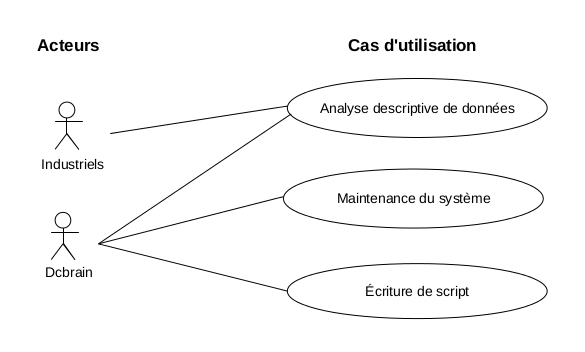
\includegraphics[scale=0.8]{diagCU.png}\end{center}
				
			\subsubsection{Analyse descriptive de données}
				DCbrain et les industriels eux-mêmes lancent des ADD sur l'applet à partir d'un fichier CSV au bon format.\\
				Sur une applet s'exécutant dans un navigateur, l'acteur importe son fichier s'il est au bon format - retenter sinon. Il peut ainsi consulter un échantillon du jeu de données brut et deux options sont maintenant disponibles.\\
				L'acteur peut naviguer pour consulter soit une description préliminaire du fichier, soit les données étant mal typées et donc non analysables.\\
				Le déroulement type se poursuit en attribuant un rôle aux colonnes du fichier puis à la sélection de l'une d'elles pour lancer son analyse si l'ensemble de données n'est pas vide.\\
				L'acteur va enfin consulter les résultats de l'ADD et décider de lancer une autre analyse sur le même fichier, importer un autre fichier, ou sauvegarder les résultats en local.
				
			\subsubsection{Ecriture de script}
				Les développeurs de DCbrain utilisent les API pour automatiser des tâches ou bien interfacer le produit avec un autre système.\\
				Il sera nécessaire d'installer sur le bureau de travail les paquets des API pour ensuite pouvoir les importer et les utiliser dans un code.\\
				La démarche d'installation, les spécifications des outils des interfaces et leur description sera détaillée dans une documentation.
				
			\subsubsection{Maintenance du système}
				Les développeurs manipulent le code source pour étendre et mettre à jour le système. La démarche sera effectuée lorsque le produit devra être modifé pour des raisons de compatibilité avec le langage et les navigateurs, ou alors pour une extension des fonctionnalités.\\
				Le nouveau modèle est d'abord conçu. On identifie les éléments à modifier et/ou l'on étudie les fonctionnalités del'extension.\\
				Les spécifications seront alors réécrites si nécessaire pour ensuite développer et déployer le système mis à jour.\\
				\textbf{Remarque :} à l'issue de la conception du nouveau modèle, une étude des coûts peut être utile pour déterminer s'il faut poursuivre la maintenance.
				
		\subsection{Organigramme et fonctionnalités des modules}
		
			\subsubsection{Organigramme et données échangées}
			
				\begin{figure}[H]
				\begin{tikzpicture}
				\begin{scope}[xscale=2,yscale=1.5]	
					\node (IW) at (0,5) [rectangle,draw,text depth=3cm,minimum width=16cm,minimum height=4cm,font=\textbf\Large] {\begin{tabular}{c}Interface web\end{tabular}};
					\node (F2) [rectangle,draw,dashed] at ([yshift=0.4cm]IW.center) {\begin{tabular}{c}Fenêtre rôle et choix colonne \end{tabular}};
					\node (F1) [rectangle,draw,dashed] at ([xshift=-4cm]F2.east) {\begin{tabular}{c}Fenêtre choix fichier\end{tabular}};
					\node (F3) [rectangle,draw,dashed] at ([xshift=4.1cm]F2.west) {\begin{tabular}{c}Fenêtre résultats ADD\end{tabular}};
					\node (MAIN) [rectangle,draw,dashed,below=of F2.south,yshift=0cm] {\begin{tabular}{c}Gestion des flux\end{tabular}};

				
					\node (API1) at (-2.5,0) [rectangle,draw,fill=blue!25,text depth=-3.5cm,minimum width=5cm,minimum height=5cm,font=\textbf\Large] {\begin{tabular}{c}API 1\\Chargement des données\end{tabular}};
					\node (VERIF) [rectangle,draw,dashed,fill=white] at ([yshift=1cm]API1.center){\begin{tabular}{c}Vérification format\\fichier\end{tabular}};
					\node (ANALYS) [rectangle,draw,dashed,fill=white,below=of VERIF.south,yshift=0.5cm] {\begin{tabular}{c}Analyse contenu\\fichier\end{tabular}};
				
					\node (API2) at (2.5,0) [rectangle,draw,fill=blue!25,text depth=-5cm,minimum width=5cm,minimum height=6.5cm,font=\textbf\Large] {\begin{tabular}{c}API 2\\Analyse descriptive des données\end{tabular}};
					\node (ADD1) [rectangle,draw,dashed,fill=white] at ([yshift=1.7cm]API2.center){\begin{tabular}{c}ADD qualitatives\end{tabular}};
					\node (ADD2) [rectangle,draw,dashed,fill=white,below=of ADD1.south,yshift=0.5cm] {\begin{tabular}{c}ADD quantitatives\\discrètes\end{tabular}};
					\node (ADD3) [rectangle,draw,dashed,fill=white,below=of ADD2.south,yshift=0.5cm] {\begin{tabular}{c}ADD quantitatives\\continues\end{tabular}};
				
					\draw[-triangle 45] (F1.south east) -- node[anchor=south,left]{11} (MAIN.north west);
					\path[->,>=stealth'] (MAIN) edge[bend left=10] node[anchor=south,left]{12} (F2);
					\path[->,>=stealth'] (F2) edge[bend left=10] node[anchor=south,right]{13} (MAIN);
					\path[->,>=stealth'] (MAIN) edge[bend left=10] node[anchor=south,right]{14} (F3);
					\path[->,>=stealth'] (F3) edge[bend left=10] node[anchor=south,right]{15} (MAIN);
				
					\draw[-triangle 45] (MAIN.south west) -- node[anchor=south,left] {1} (VERIF.100);
					\draw[-triangle 45] (VERIF.80) -- node[anchor=south,right] {2} (MAIN.197);
					\draw[-triangle 45] (MAIN.210) |- node[anchor=south,left] {3} (ANALYS.5);
					\draw[-triangle 45] (ANALYS.355) -| node[anchor=south,below] {4} (MAIN.215);			
				
					\draw[-triangle 45] (MAIN.south east) -- node[anchor=south,right] {5} (ADD1.80);
					\draw[-triangle 45] (ADD1.110) -- node[anchor=south,left] {6} (MAIN.343);
					\draw[-triangle 45] (MAIN.335) |- node[anchor=south,right] {7} (ADD2.175);
					\draw[-triangle 45] (ADD2.185) -| node[anchor=south,below] {8} (MAIN.330);				
					\draw[-triangle 45] (MAIN.290) |- node[anchor=north,right] {9} (ADD3.175);
					\draw[-triangle 45] (ADD3.185) -| node[anchor=south,below] {10} (MAIN.270);
				
				\end{scope}
				%Légende
				\begin{scope}
					\node (LEGENDE) at (-7,-5) {\textbf{Légende :}};
					\node (FAMILLE) at (-4.5,-5) [rectangle,draw] {\begin{tabular}{c}Famille\end{tabular}};
					\node (MODULE) at (-2,-5) [rectangle,draw,dashed] {\begin{tabular}{c}Module\end{tabular}};
					\path[->,>=stealth'] (0.5,-5.3) edge[bend left=0] node[anchor=south,above]{informations transmises} (3,-5.3);
				\end{scope}
				\end{tikzpicture}
				\caption{Organigramme des différents modules du logiciel}\label{fig:M1}
				\end{figure}
				
				\textbf{Notes :}\\
				(1) Fichier CSV : lancement de la vérification de son format\\
				(2) Code d'erreur : fichier OK ou ERREUR\\
				(3) Fichier CSV : lancement de l'analyse de son contenu\\
				(4) \textbf{structure 1} : contenant les données du fichier, le nombre de lignes et le nombre de colonnes (connus à partir de la taille de la structure)\\
				\hspace*{1.5em} \textbf{structure 2} : contenant 3 informations sur chaque colonne : le type, le rôle et les positions des données erronées ou manquantes\\
				(5) Ensemble de données de type qualitatif\\
				(6) Erreur ou effectifs, effectifs cumulés, fréquences, fréquences cumulées, diagramme en secteur, histogramme\\
				(7) Ensemble de données de type quantitatif discret\\
				(8) Erreur ou indicateurs de tendance central, de dispersion et de forme, les anomalies, la distribution des données, un diagramme à moustaches\\
				(9) Ensemble de données de type quantitatif continu\\
				(10) Même données que (8)\\
				(11) Chemin du fichier CSV importé \\
				(12) Informations du (4) et ensemble de données contenu dans le fichier CSV \\
				(13) Signal de validation du choix de la colonne, et noms des colonnes\\
				(14) Envoi des résultats d'analyses de (6), (8) et (10)\\
				(15) Signal de contrôle : demande d'exportation des résultats de l'ADD, analyse d'une autre colonne, ou importation d'un autre fichier\\
			
			\subsubsection{Format du fichier CSV}
				Le format du fichier est établi par DCbrain. Son contenu est décrit par des colonnes aux types prédéfinies :
				\begin{itemize}
				\item Timestamp : jour/mois/année	\lstinline!heure:minute:seconde!
				\item Père : nom du noeud
				\item Enfant : nom du noeud
				\item Mesure (unité) : Valeur
				\end{itemize}
				\textbf{Remarques :} le graphe de flux utilisé par DCbrain pour analyser les réseaux de ses clients est orienté, d'où l'utilisation des éléments \textit{Père - Enfant}. Ceux-ci permettent de repérer de quelle connexion on parle.\\
				Les colonnes \textit{Mesure} renseignent sur les données mesurées sur une connexion à un temps donné.
				
			\subsubsection{Fonctionnalités des modules}
			\begin{description}[style=unboxed,leftmargin=0.2cm]
			
				\item\textbf{1. API 1 - Chargement des données}
				\begin{enumerate}
					\item Module Vérification format fichier :\\
					Ce module va vérifier le fichier fourni en entrée en plusieurs points :
					\begin{itemize}
						\item l'ouverture du fichier a réussi
						\item le fichier est un CSV contenant du texte brut non formaté (pas de mise en forme avec des balises ou autres)
						\item le fichier est accessible en lecture
					\end{itemize}
					\textbf{Critère de satisfaction : } le fichier est bien ouvert, accessible en lecture et ne contient que du texte brut.
				
					\item Module Analyse contenu fichier :\\
					Ce module comprend deux fonctionnalités principales :
					\begin{itemize}
						\item Lecture du contenu du fichier CSV :\\
						On initialise une première structure (\textbf{structure 1}) pour y sauvegarder le contenu du fichier.\\
						On lit ligne par ligne des caractères du fichier. A chaque fois qu'on détecte un caractère de séparation (une virgule, un point-virgule ou une tabulation), on stocke les caractères lus (la donnée) dans la structure.\\
						Cette fonctionnalité fournit la \textbf{structure 1} contenant les données du fichier, le nombre de lignes et le nombre de colonnes (connus à partir de la taille de la structure).\\
						\textbf{Critère de satisfaction : } l'ensemble des entrée du fichier sont renseignées dans une structure (donc exploitables).
						
						\item Descriptions préliminaires des données de chaque colonne du fichier CSV :\\
						On initialise une deuxième structure (\textbf{structure 2}) pour y stocker des informations sur chaque colonne.\\
						On lit une par une les données de chaque colonne. On vérifie le type de la donnée en le comparant au type attendu. Si le type ne correspond pas, on signale dans la structure que la colonne contient une donnée erronée ou manquante (repérée par sa position dans la colonne). A la fin du parcours d'une colonne, on pourra lui attribuer un rôle/nom.\\
						Cette fonctionnalité fournit donc la \textbf{structure 2} contenant 3 informations sur chaque colonne : le type, le rôle et les positions des données erronées ou manquantes.\\
						\textbf{Critère de satisfaction : } pour chaque colonne, on connaît son type, son rôle et les éventuels données erronées.
					\end{itemize}
					Ce module va donc fournir les deux structures \textbf{structure 1} et \textbf{structure 2} décrites ci-dessus.
				\end{enumerate}
				~\\
				\item\textbf{2. API 2 - Analyse descriptive de données}
				\begin{enumerate}
					\item Module ADD qualitatives :
						\begin{itemize}
						\item effectifs, effectifs cumulés
						\item fréquence et fréquence cumulée
						\item représentations graphiques : diagramme en secteur, histogramme
						\end{itemize}
					\item Module ADD quantitatives discrètes :
						\begin{itemize}
						\item tendance centrale : moyenne, médiane
						\item dispersion : quantiles, variance et écart-type
	-					\item anomalies : boîte à moutaches de Tukey
						\item forme (symétrie) : coeff de Pearson ou coeff de Yule
						\item forme (aplatissement) : coeff de Fisher
						\item représentations graphiques : distribution, cumulatif,  boîte à moustaches, ...
						\end{itemize}
					\item Module ADD quantitatives continues :
						\begin{itemize}
						\item découpage en classe selon une précision définie
						\item découpage en classe selon une précision par défaut (échelle définie après un parcours des valeurs)
						\item représentations graphiques : distribution, boîte à moustaches, ...
						\end{itemize}
				\end{enumerate}
				~\\
				\item\textbf{3. Interface web}
				\begin{enumerate}
					\item Module Gestion des flux :
						\begin{itemize}
						\item Lancement de l'application et exécution continue.
						\item Gestion des branchements : exécution normale ou arrêts pour cause d'erreur.
						\item Interface entres les différentes fonctionnalités : communique les données nécessaires entre les modules.
						\end{itemize}
						
					\item Module Fenêtre choix fichier :
						\begin{itemize}
						\item Récupération un fichier CSV.
						\item Validation du choix pour passer à la prochaine fenêtre (En renseignant son chemin dans le système de fichier, ou de la manière d'un Drag \& Drop).\\
						\textbf{Critère de satisfaction : } le fichier devra être chargé  et devra correspondre à la demande.
						\end{itemize}
						
					\item Module Fenêtre rôle et choix colonne :
						\begin{itemize}
						\item Affichera le nombre de lignes/colonnes contenu dans le CSV.\\
							\textbf{Critère de satisfaction : } affiche le bon nombre de lignes et de colonnes.
						\item Affichera le titre du fichier.\\
							\textbf{Critère de satisfaction : } affiche le bon titre du fichier.
						\item Affichera un échantillon du contenu du CSV (environ les 1000 premières lignes) avec un système de scroll.\\ 
							\textbf{Critère de satisfaction : } l'affichage de l'échantillon doit bien se faire sur les 1000 premières valeurs et doivent bien correspondre bien correspondre au contenu du fichier. 
						\item Affichage des lignes erronés (numéro de la ligne + contenu + type d'erreur).\\
							\textbf{Critère de satisfaction : } doit bien afficher les lignes contenant les erreurs, le contenu et leur type de façon précise.
						\item Mise en place d'un système de navigation sous forme d'onglet (Onglet erreurs, onglet échantillon,...). Cela permettra d'éviter que la fenêtre contienne trop d'informations.\\
							\textbf{Critère de satisfaction : } le système de navigation doit être lisible et pratique sans trop charger la fenêtre.
						\item L'Utilisateur devra sélectionner la colonne avec un clic, puis pourra lancer l'analyse sur celle-ci. \\
							\textbf{Critère de satisfaction : } sélection de la colonne doit bien se faire + lancement possible après la sélection.
						\end{itemize}
					
					\item Module Fenêtre résultats ADD :
						\begin{itemize}
						\item La fenêtre affichera les résultats de l'étude qualitative (Médiane, Quantile et anomalie) d'une part et de l'étude quantitative (Histogramme et Diagramme de secteur) d'autre part.\\
						\textbf{Critère de satisfaction : } résultats conformes + diagramme bien dessiné. 
						\item Une fonctionnalité pour lancer l'exportation des résultats sera disponible (Écriture dans un nouveau fichiers).
						\end{itemize}
					\end{enumerate}
				
			\end{description}
			
			\textbf{Remarque :} en ce qui concerne les critères de satisfaction de l'ADD, puisqu'il s'agit d'un domaine scientifique, le système devra fournir des résultats conformes aux techniques de ce domaine.
	
	
	\section{Exigences non fonctionnelles}
		\subsection{Interface utilisateur du produit}
		
			\subsubsection{Exigences d’apparence} 
			Le produit devra adopter une apparence simple, agréable et devra être facile à comprendre dès sa première prise en main.
			Le maître d’ouvrage a émis le souhait d’avoir de l’Anglais comme langue utilisée pour l’affichage textuel.

			\subsubsection{Exigences de style}
			Le produit doit fournir une interface graphique interactive et intuitive à l'utilisateur.

		\subsection{Utilisabilité}
		Le produit devra être simple d’utilisation et facile à comprendre dès sa première prise en main, pour ne pas soumettre une formation concernant la manipulation du produit aux futurs utilisateurs.
		

		\subsection{Exigences de performance} 
		Les exigences de performance du futur produit concerne la latence acceptable que devra avoir l'application. Ici la durée de réponse de l’affichage d’un CSV, ou d’une requête concernant l’analyse de données venant de l’utilisateur ne devra pas être trop longue, le client a suggérer que cette attente devra être de l’ordre de la minute. En ce qui concerne le temps de passage d'une fenêtre à l'autre (choix de(s) colonne(s) pour l'exécution d'une analyse statistique, affichage de la fenêtre d'erreurs, lors du choix du méthode d’affichage des résultats,..), l’application devra répondre de manière fluide. 

		\subsection{Précision et exactitude}
			Lors de l'analyse des données, les résultats sur la Variance et la Moyenne doivent être calculée de façon très précise car elles vont servir de base dans d’autres calculs statistiques. Les autres valeurs calculées peuvent être les plus précises possible mais ces valeurs vont servir pour l'interprétation afin mieux comprendre ce qui se passe sur le réseau.

		\subsection{Maintenabilité du projet}
		Le produit doit pouvoir être maintenu par ses utilisateurs finaux ou par des développeurs qui ne sont pas les développeurs d’origines, dans le cas où DCbrain souhaiterait ajouter de nouvelles méthodes d’analyses descriptives ou de nouveaux procédés pour afficher les résultats de manière graphique afin de satisfaire les exigences de leurs clients.\\
		
		Le produit devra permettre l'insertion d'éventuels API supplémentaires, tel que l'ADD multidimensionnelle qui utilisera l'API de l'ADD unidimensionnel dans le but de fournir des descriptions statistiques plus poussées pour obtenir une meilleur vue d'ensemble sur les données collectées. Mais encore l'insertion de technique d'analyse de graphe dans le but d'obtenir des informations sur ces derniers.
		
		\subsection{Sécurité} 
			\subsubsection{Accès au système}
			Le produit final étant une application web, l'accès au système se fera à partir d'un navigateur web pour les utilisateurs. L'accès au produit sera défini grâce à un mécanisme d'adressage (path) dans un système de gestion de fichiers.
			\subsubsection{Intégrité}
			Le produit manipulera des données fiables. Les données ne représenteront pas de risques pour l'environnement et l'utilisateur du produit final.
			\subsubsection{Protection des données à caractères personnel}
			Le produit ne devant pas faire appel aux données à caractères personnel des utilisateurs, ne devra donc aucunement altérer ou supprimer de telles données.		
		
	\section{Autres aspects du projet}
		\subsection{Question ouvertes}
			La question de l'esthétisme et la présentation des résultats est laissée ouverte puisqu'il n'y a pas de réponse arrêtée à ce sujet. Le tout est d'avoir une approche prenant en compte les utilisateurs pour savoir quelles vues faciliteront l'interprétation des analyses.
			
		\subsection{Choix du langage}
				D'un point de vue technique, le choix des langages de programmation utilisés pour le développement du produit est justifié par les contraintes et les exigences définies précédemment.\\
		La contrainte 1 (fournir une application web) et la contrainte 2 (compatibilité avec ADD) nous permettent de nous fixer sur le choix du langage : \textbf{\textit{Python}}.\\
		D'une part, ce langage est compatible avec le développement d'applications web grâce aux nombreuses bibliothèques web qui permettent cela, par exemple \textbf{\textit{Django}}. D'autre part, Python est doté de plusieurs modules permettant d'effectuer du calcul scientifique sur des données et donc de l'analyse de données, par exemple l'ensemble des outils mis à disposition par le \textbf{\textit{Projet SciPy}}.\\
		De plus, puisque le produit doit être une applet intégrée dans une page web pour s'exécuter, on va donc avoir recours à des langages de balisage comme \textbf{\textit{HTML}} pour la présentation et \textbf{\textit{CSS}} pour la mise en forme de ces pages web.

		\subsection{Tâche à faire}
			\subsubsection{Étapes}
			Le développement du produit se décompose en deux étapes :
				\begin{itemize}
				\item Spécifications
				\item Développement de l'application
				\item Compte-rendu
				\end{itemize}
				
			\subsubsection{Phases de développement}
				\begin{itemize}
				\item Build
				\item Développement des fonctionnalités
				\item Développement des tests
				\item Écriture de la documentation
				\item Exécution des tests et correction éventuelle du code (debug)
				\end{itemize}
				
				\textbf{Remarque} : Ces étapes ne sont pas effectuées séparément, il sera avantageux de les réaliser en même temps. L'intensité de travail sur chacune des phases va varier tout au long du projet.
				

		\subsection{Contrôle de la finalisation}
			La qualité de l'applet sera étudiée selon plusieurs niveaux :
			\begin{enumerate}
			\item Le test des fonctionnalités du système.
			\item La vérification de la satisfaction des exigences.
			\item Une mesure de la conformité du produit avec les spécifications.
			\end{enumerate}
			
		\subsection{Estimation des coûts}
		
			\subsubsection{Tableau des coûts}
			\begin{center}\begin{longtable}{|>{\centering}m{3cm}|>{\centering}m{4cm}|>{\centering\arraybackslash}m{7cm}|}			
				\hline \multicolumn{1}{|c|}{\textbf{Module}} & \multicolumn{1}{c|}{\textbf{Nombre de lignes}} & \multicolumn{1}{|c|}{\textbf{Justification}} \\
				\hline 	Gestion des flux & 15 & Mise en forme du main et appel de l'application \\
				\hline 	Fenêtre choix fichier & 10 + 20 & Fonctions pour : Drag\& Drop + Système de fichiers\\
				\hline 	Fenêtre rôle et choix colonne & 5 + 20 + 10 + 10 + 20 & Communication avec le module application + Affichage de l'interface+ lecteurs des valeurs + 	affichage des valeurs \\
				\hline 	Fenêtre résultats ADD & 10 + 3* 30 &  Envoie d'informations au module application + Construction des graphe pour l'ADD pour les 3 types d'analyse \\
				\hline  ADD qualitatives  & 20 + 20*3 & Application des formules pour les calculs de fréquences et d'effectifs + calcul des valeurs pour la construction de 3 graphes \\
				\hline 	ADD quantitatives discrètes & 60 + 20*2 & Application des formules attaché à l'analyse quantitative discret + calcul des valeurs pour la construction de 2 graphes \\
				\hline 	ADD quantitatives continu & 20 + 10 + 10 + 5 + 20*2 & Parcours + choix précision classe d'intervalle + écriture + communication avec les modules+ calcul des valeurs pour la construction de 2 graphes\\
				\hline 	Vérification format fichier & 30 & Ouverture fichier + vérification si ouverture en lecture + présence de texte formaté ou non\\
				\hline 	Analyse contenu fichier & 20 + 5 + 25 + 10 &  Recopie et vérification + initialisation de la structure+ Parcours du fichiers avec condition + Fonction pour donner nom et type de colonne\\
				\hline \textbf{Coût Total} & \textbf{565} & \textbf{Estimation totale du coût}\\
				\hline 	
				\end{longtable}\vspace{1em}\end{center}
			
			\subsubsection{Tableau répartition des tâches}
			\begin{center}\begin{longtable}{|>{\centering}m{5cm}|>{\centering}m{2cm}|>{\centering}m{2cm}|>{\centering}m{2.5cm}|>{\centering\arraybackslash}m{1cm}|}			
			\hline \multicolumn{1}{|c|}{\textbf{Module}} & \multicolumn{1}{c|}{\textbf{Malek}} & \multicolumn{1}{ c|}{\textbf{Sonny}} & \multicolumn{1}{c|}{\textbf{Jean-Didier}} & {\textbf{Total}} \\
			\hline 	Gestion des flux & ~ & ~ & x & 1\\
			\hline 	Fenêtre choix fenêtre & ~ & ~ & x & 1\\
			\hline 	Fenêtre rôle et choix colonne & x & ~ & ~ & 1\\
			\hline 	Fenêtre résultats ADD & ~ & x & ~ & 1\\
			\hline  ADD qualitatives & ~ & ~ & x & 1\\
			\hline 	ADD quantitatives discrètes & ~ & x & ~ & 1\\
			\hline 	ADD quantitative continues &  ~ & x & ~ & 1\\
			\hline 	Vérification format fichier & x & ~ & ~ & 1\\
			\hline 	Analyse contenu fichier & x & ~ & ~ & 1\\
			\hline
			\end{longtable}\vspace{1em}\end{center}
			
			
		\subsection{Documentation utilisateur et formation}
			Le produit final ne nécessitera pas de formation pour apprendre sa manipulation. Mais une documentation utilisateur sera fournie en même temps que le produit, dans lequel sera détaillé les consignes d'installation et d'utilisations.
			
	\section*{Conclusion}
		Les contraintes et les exigences du projet sont facteurs qui nous ont permis de choisir le langage de programmation. Cependant, cette étape a abouti à deux langages potentiels Java et Python. Notre choix s'est finalisé avec Python, c'est un langage plus préconisé par les startups pour construire des applications. Java, lui, est utilisé par des entreprises pouvant se permettre de déployer plus de moyens pour le développement et la maintenance du système.
		
		\paragraph{} Pour finir, il est intéressant de mentionner les difficultés rencontrées au cours de l'élaboration du cahier des charges.\\
		Le plus difficile a été pour nous d'apprendre une nouvelle démarche tout en la pratiquant dans un projet de grande ampleur pour des étudiants. Ceci entraîne des efforts supplémentaires au niveau de l'organisation et de la gestion des délais à cause du double travail exigé.\\
		Cela dit, ce premier travail nous a permis à la fois de réaliser l'impact des efforts individuels et collectifs pour mettre à bien un travail qui semble \textit{à priori} difficile, mais aussi d'aborder de nouveaux projets avec une approche plus pragmatique.\\
	
	\section*{Bibliographie/sitographie ADD}
	\begin{itemize}
		\item http://www.math.univ-toulouse.fr/~baccini/zpedago/asde.pdf
		\item http://www.math.univ-toulouse.fr/~besse/Wikistat/pdf/st-l-des-uni.pdf
		\item http://iml.univ-mrs.fr/~reboul/cours2.pdf
		\item https://hal.archives-ouvertes.fr/halshs-00287751/document
		\item Wikipédia : Données aberrantes
		\item Exploration de données et méthodes statistiques - Ellipses - Lise Bellanger, Richard Tomassone
		\item Statistique théorique et appliquée: 1. Statistique descriptive et base de l'inférence statistique - 3e édition - de boeck - Pierre Dagnélie
	\end{itemize}
\end{document}
